\documentclass{beamer}
\usetheme{Darmstadt}

\usepackage{color}
\usepackage{listings}
\usepackage{graphicx}

\setbeamertemplate{frametitle}[default][center]

\title{Utilizing Crowd Intelligence for Online Detection of Emotional Distress}
\subtitle{Master's Thesis Presentation}
\author[Siddhant Goel]{Siddhant Goel\\{\small Advisor: Han Xiao\\Supervisor: Prof. Dr. Claudia Eckert}}
\institute{
Chair for IT Security\\
Technische Universit\"at M\"unchen
}
\date{\today}

\begin{document}
    \begin{frame}[plain]
        \titlepage
    \end{frame}
    
    \begin{frame}
        \frametitle{Outline}
        \begin{itemize}
            \item{
            Introduction
            \begin{itemize}
                \item{Introduction}
                \item{Problem Definition}
            \end{itemize}
            }
            \item{
            Theoretical Background
            \begin{itemize}
                \item{Machine Learning and Text Classification}
                \item{Support Vector Machines}
                \item{Ensemble Learning methods}
            \end{itemize}
            }
            \item{
            Experimental Results
            \begin{itemize}
                \item{Experiments}
                \item{Results}
            \end{itemize}
            }
            \item{Conclusion}
        \end{itemize}
    \end{frame}
    
    \begin{frame}
        \begin{center}
            \textbf{Introduction}
        \end{center}
    \end{frame}
    
    \begin{frame}
        \frametitle{Introduction}
        \begin{itemize}
            \item{Millions of people die every year because of suicide}
            \item{Most people are between 15 to 29 years old}
            \item{Rise of social media - Twitter, Facebook, Reddit, Wordpress}
            \item{Reddit - ``/r/happy'' and ``/r/suicidewatch''}
            \item{People are not afraid of posting their inner feelings on the web}
        \end{itemize}
    \end{frame}
    
    \begin{frame}
        \frametitle{Introduction}
        \begin{figure}
            \centering
            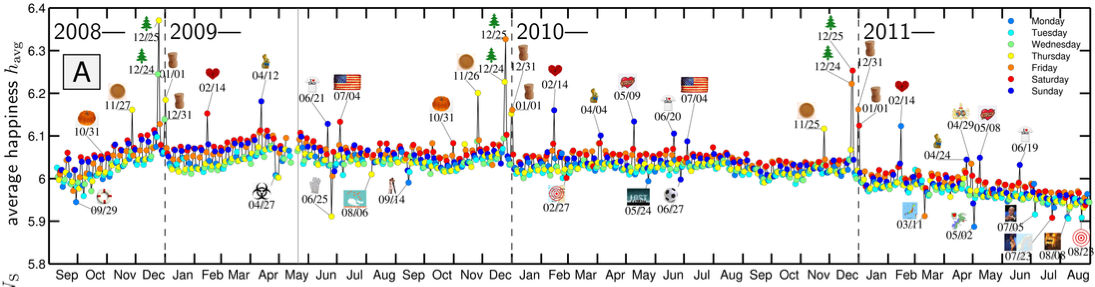
\includegraphics[width=\textwidth]{figures/twitter_happiness.png}
            \caption{Happiness on Twitter as a function of time}
        \end{figure}
        \begin{itemize}
            \item{Study conducted in 2011}
            \item{46 billion words collected over 33 months}
            \item{Negativity on Twitter has been on the rise}
            \item{Words include \emph{death}, \emph{hate}, and even \emph{suicide}}
        \end{itemize}
    \end{frame}
    
    \begin{frame}
        \frametitle{Motivation}
        \begin{figure}
            \centering
            
\includegraphics[width=0.5\textwidth]{figures/twitter_kcs.png}
        \end{figure}
        \begin{itemize}
            \item{Last tweet of Twitter user ``@CapitalSTEEZ\_'' \footnote{\url{http://twitter.com/CapitalSteez\_}}}
            \item{Some accounts have lots of followers, some don't}
            \item{Lives can be saved if there is a surveillance system of suicide}
            \item{Public sentiment information available on the web + No analysis possible = Disconnect}
        \end{itemize}
    \end{frame}
    
    \begin{frame}
        \frametitle{Problem Definition}
        \begin{itemize}
            \item{Evaluate machine learning algorithms (including support vector machines and ensemble learning methods) that can be used for text classification}
            \item{
            Build a web based system that can
            \begin{itemize}
                \item{tap into crowd intelligence to incrementally improve the classifiers}
                \item{detect content on the web that indicates that its author is depressed or suicidal}
            \end{itemize}
            }
        \end{itemize}
    \end{frame}
    
    \begin{frame}
        \begin{center}
            \textbf{Theoretical Background}
        \end{center}
    \end{frame}
    
    \begin{frame}
        \frametitle{Machine Learning}
        \begin{itemize}
            \item{Algorithms that can learn from data}
            \item{Construct a model from a given dataset, and then perform the required task on another dataset}
            \item{\textbf{Supervised Learning} - Train the models on the training data, and predict on the test data}
            \item{\textbf{Unsupervised Learning} - No distinction between training and test data}
        \end{itemize}
    \end{frame}
    
    \begin{frame}
        \frametitle{Text Classification}
        \begin{itemize}
            \item{Subset of machine learning algorithms (we focus on supervised text classification)}
            \item{Given some pieces of text, put future pieces of text into two or more categories}
            \item{Dataset ${(\mathbf{x_n}, y_n)}_{n = 1}^{N}$ containing N instances}
            \item{Each instance $(\mathbf{x_n}, y_n)$ is of the form $[(x_{n, 1}, x_{n, 2}, ..., x_{n, D}), y_n]$}
            \item{Supervised learning - calculate $y_n$ of test data given information about $y_n$ from training data}
            \item{Unsupervised learning - calculate $y_n$ given only information about $\mathbf{x_n}$}
        \end{itemize}
    \end{frame}
    
    \begin{frame}
        \frametitle{Support Vector Machines}
        \begin{itemize}
            \item{Fairly popular class of algorithms in binary classification}
            \item{Given training data in $D$ dimensional space, find a decision boundary (hyperplane) that separates the two classes}
            \item{Maximize the distance of the boundary from any data point}
            \item{Decision function depends on a (usually small) subset of points called support vectors}
            \item{Distance function between two points is expressed using a kernel function}
        \end{itemize}
    \end{frame}
    
    \begin{frame}
        \frametitle{Linear kernel SVM}
        \begin{figure}
            \centering
            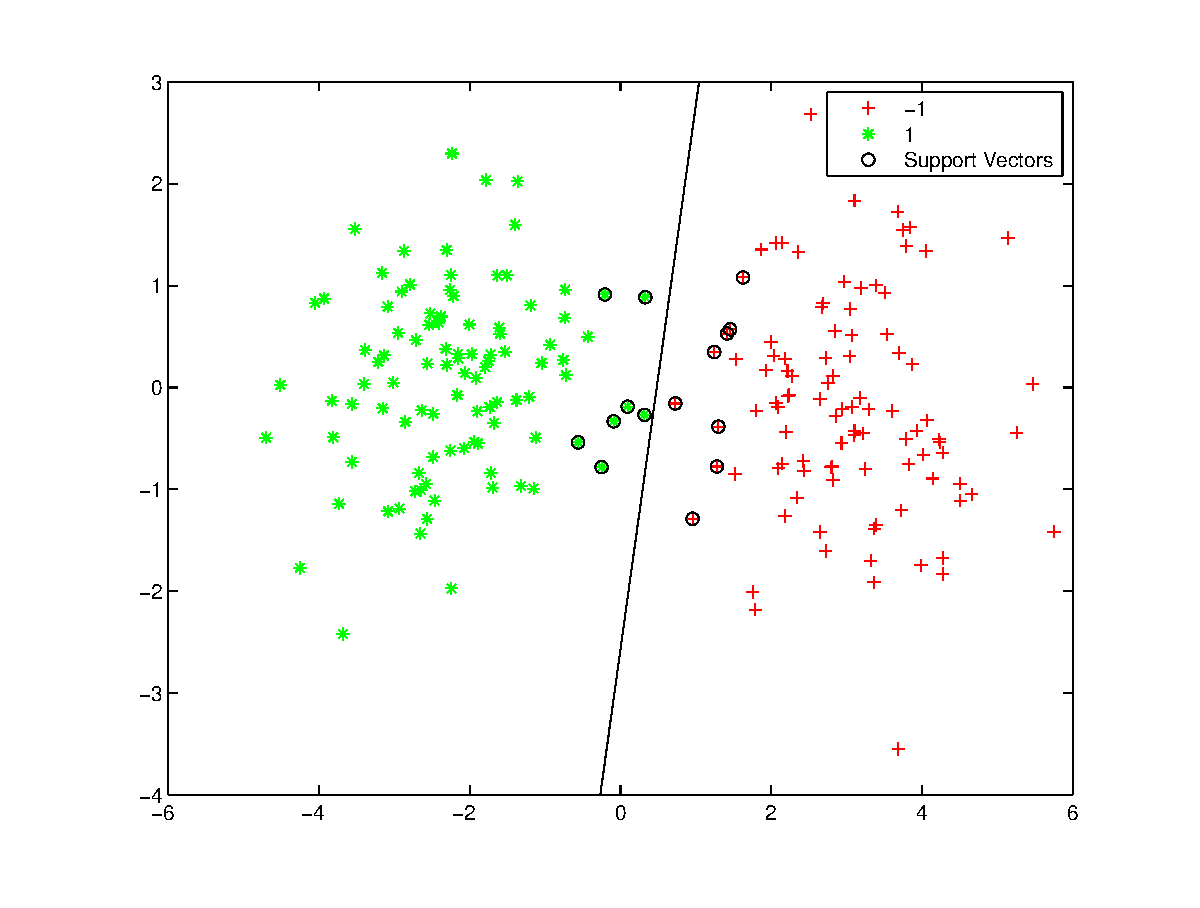
\includegraphics[width=0.5\textwidth]{figures/svm_linear_classification.eps}
            \caption{Classifying two subsets of a dataset using a linear kernel SVM}
        \end{figure}
    \end{frame}
    
    \begin{frame}
        \frametitle{Kernel functions}
        \begin{figure}
            \centering
            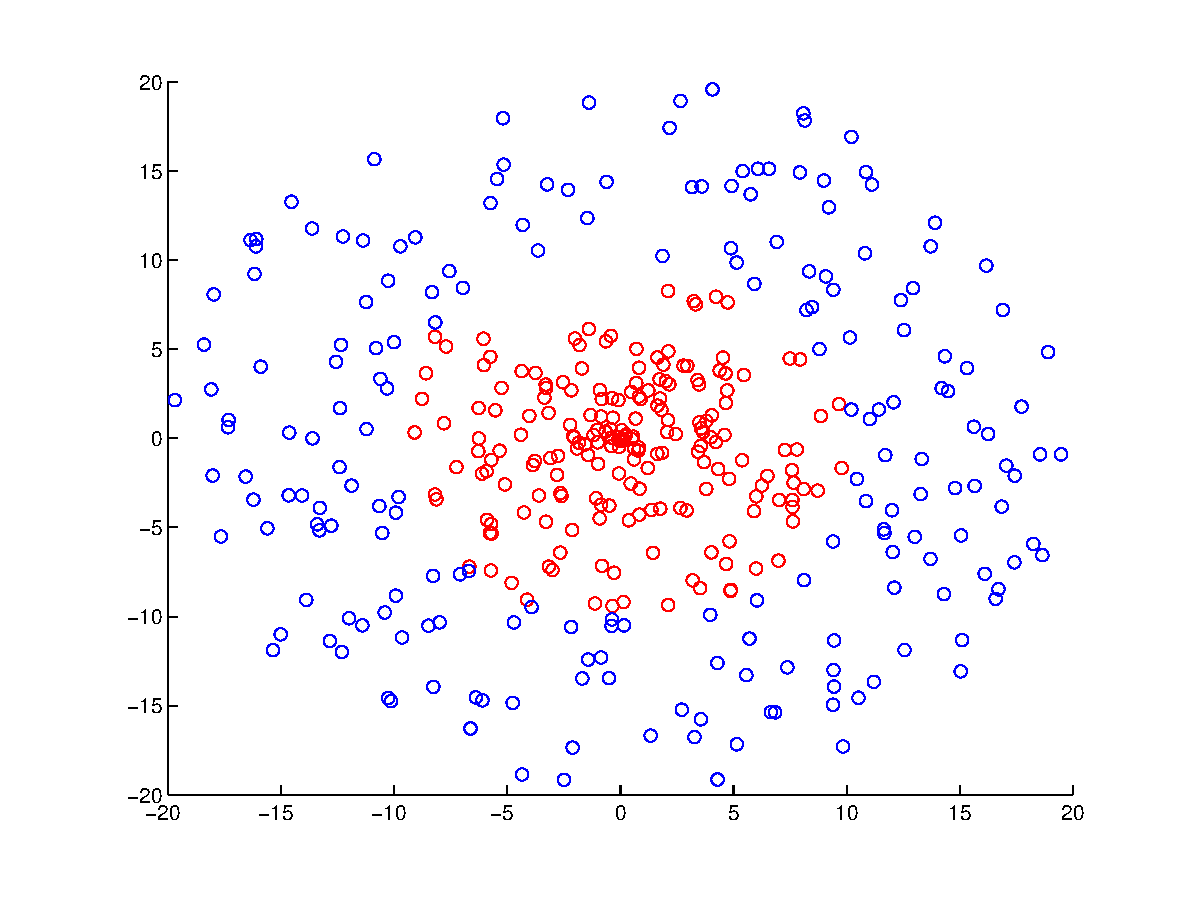
\includegraphics[width=0.5\textwidth]{figures/svm_non_linear_data.eps}
            \caption{A dataset that cannot be classified using a linear kernel SVM}
        \end{figure}
    \end{frame}
    
    \begin{frame}
        \frametitle{Kernel functions}
        \begin{figure}
            \centering
            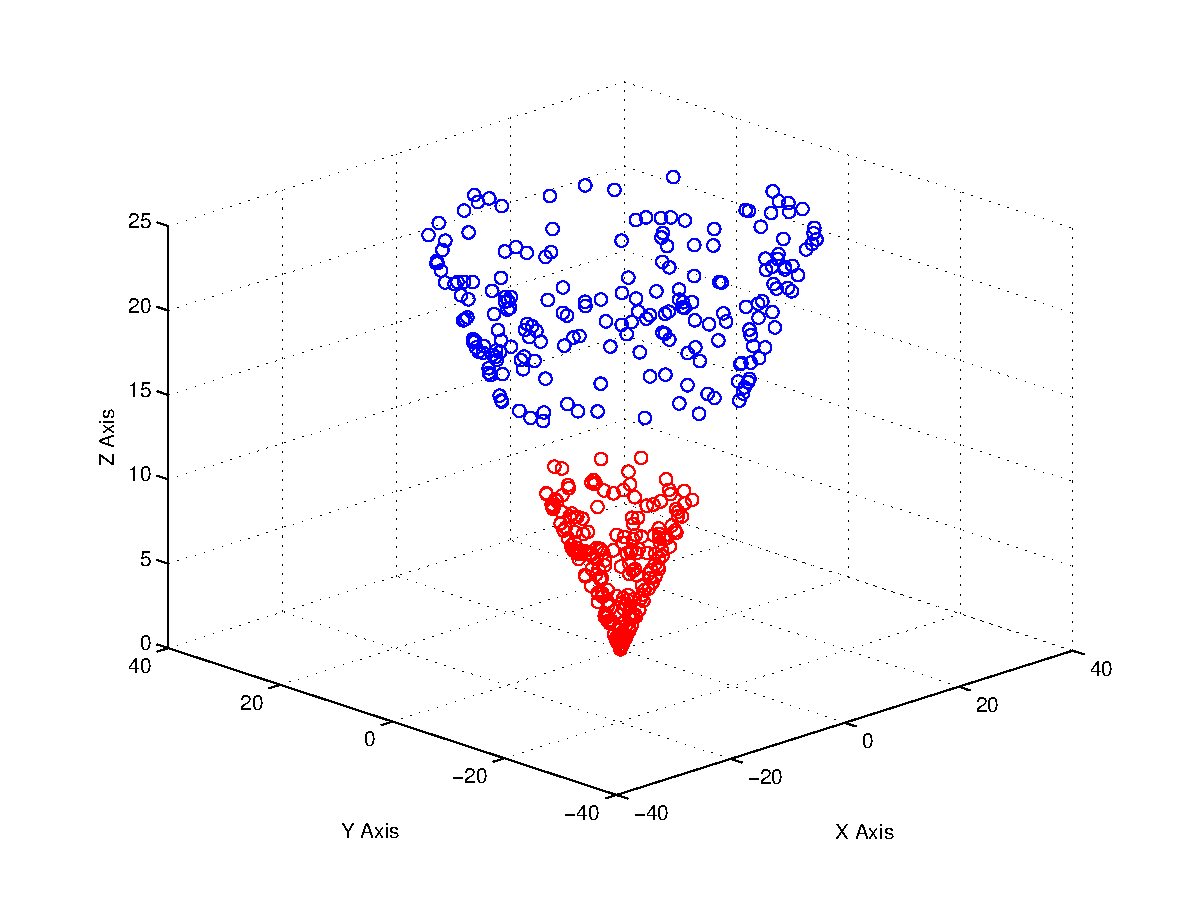
\includegraphics[width=0.5\textwidth]{figures/svm_non_linear_data_3d.eps}
            \caption{Add the third dimension as $\sqrt{x_1^2 + x_2^2}$ to transform the dataset into 3D}
        \end{figure}
    \end{frame}
    
    \begin{frame}
        \frametitle{Ensemble Learning}
        \begin{itemize}
            \item{Class of machine learning methods that combine models to obtain better predictions}
            \item{Performance not guaranteed to be better than constituent classifiers}
            \item{Ensemble methods still usually outperform individual classifiers}
        \end{itemize}
    \end{frame}
    
    \begin{frame}
        \frametitle{Bagging}
        \begin{itemize}
            \item{Combine $M$ classifiers to form a single classifier}
            \item{To predict, obtain predictions from all constituent classifiers, and take majority vote}
            \item{Requirement - classifiers should change for even small changes in underlying classifiers}
            \item{
            Two main approaches for training individual classifiers
            \begin{itemize}
                \item{Sample split - each classifier is trained using a random subset of the samples}
                \item{Feature split - each classifier is trained using a random subset of the features}
            \end{itemize}
            }
        \end{itemize}
    \end{frame}
\end{document}
